\documentclass[a4paper,10pt]{article}
\usepackage{titlesec}
\usepackage{graphicx}
\usepackage{amsmath}
\usepackage[english]{babel}
\usepackage{hyperref}
\usepackage{tikz}
\usetikzlibrary{shapes,fit,patterns}
\usepackage{amssymb}
\usepackage{pifont}
\usepackage{breqn}
\usepackage[
   backend=biber,%
   bibencoding=utf8,%
   language=english,%
   style=numeric-comp,%
   sorting=nyt,%
   maxbibnames=10,%
   natbib=true%
]{biblatex}
\addbibresource{references.bib}
\graphicspath{ {./img/} }

% Add X and check marks
\newcommand{\cmark}{\ding{51}}%
\newcommand{\xmark}{\ding{55}}%

% Add subsubsubsection
\titleclass{\subsubsubsection}{straight}[\subsubsection]

\newcounter{subsubsubsection}[subsubsection]
\renewcommand\thesubsubsubsection{\thesubsubsection.\arabic{subsubsubsection}}
\renewcommand\theparagraph{\thesubsubsubsection.\arabic{paragraph}} % optional; useful if paragraphs are to be numbered

\titleformat{\subsubsubsection}
  {\normalfont\normalsize\bfseries}{\thesubsubsubsection}{1em}{}
\titlespacing*{\subsubsubsection}
{0pt}{3.25ex plus 1ex minus .2ex}{1.5ex plus .2ex}

\makeatletter
\renewcommand\paragraph{\@startsection{paragraph}{5}{\z@}%
  {3.25ex \@plus1ex \@minus.2ex}%
  {-1em}%
  {\normalfont\normalsize\bfseries}}
\renewcommand\subparagraph{\@startsection{subparagraph}{6}{\parindent}%
  {3.25ex \@plus1ex \@minus .2ex}%
  {-1em}%
  {\normalfont\normalsize\bfseries}}
\def\toclevel@subsubsubsection{4}
\def\toclevel@paragraph{5}
\def\toclevel@paragraph{6}
\def\l@subsubsubsection{\@dottedtocline{4}{7em}{4em}}
\def\l@paragraph{\@dottedtocline{5}{10em}{5em}}
\def\l@subparagraph{\@dottedtocline{6}{14em}{6em}}
\makeatother

% Set TOC depth and sections numbering
\setcounter{tocdepth}{3}
\setcounter{secnumdepth}{3}

% Fix tikz patterns
\pgfdeclarepatternformonly{south west lines}{\pgfqpoint{-0pt}{-0pt}}{\pgfqpoint{3pt}{3pt}}{\pgfqpoint{3pt}{3pt}}{
   \pgfsetlinewidth{0.4pt}
   \pgfpathmoveto{\pgfqpoint{0pt}{0pt}}
   \pgfpathlineto{\pgfqpoint{3pt}{3pt}}
   \pgfpathmoveto{\pgfqpoint{2.8pt}{-.2pt}}
   \pgfpathlineto{\pgfqpoint{3.2pt}{.2pt}}
   \pgfpathmoveto{\pgfqpoint{-.2pt}{2.8pt}}
   \pgfpathlineto{\pgfqpoint{.2pt}{3.2pt}}
   \pgfusepath{stroke}}
\pgfdeclarepatternformonly{south east lines}{\pgfqpoint{-0pt}{-0pt}}{\pgfqpoint{3pt}{3pt}}{\pgfqpoint{3pt}{3pt}}{
   \pgfsetlinewidth{0.4pt}
   \pgfpathmoveto{\pgfqpoint{0pt}{3pt}}
   \pgfpathlineto{\pgfqpoint{3pt}{0pt}}
   \pgfpathmoveto{\pgfqpoint{.2pt}{-.2pt}}
   \pgfpathlineto{\pgfqpoint{-.2pt}{.2pt}}
   \pgfpathmoveto{\pgfqpoint{3.2pt}{2.8pt}}
   \pgfpathlineto{\pgfqpoint{2.8pt}{3.2pt}}
   \pgfusepath{stroke}}
      

\begin{document}
% First page
\title{Present Wrapping Problem}
\author{Leonardo Calbi (\href{mailto:leonardo.calbi@studio.unibo.it}{leonardo.calbi@studio.unibo.it}) \\ Alessio Falai (\href{mailto:alessio.falai@studio.unibo.it}{alessio.falai@studio.unibo.it})}
\date{\today}
\maketitle
\tableofcontents
\newpage

\section*{Foreword}
The problem is presented as: given a wrapping paper roll of a certain dimension and a list of presents, decide how to cut off pieces of paper so  that all the presents can be wrapped.

Consider that each present is described by the dimensions of the piece of paper needed to wrap it. Moreover, each necessary piece of paper cannot be rotated when cutting off, to respect the direction of the patterns in the paper.

A more general case also requires the following conditions:
\begin{itemize}
   \item Rotation of the pieces of paper is allowed
   \item There can be multiple presents of the same dimensions
\end{itemize}

\section{Introduction}
The non-overlapment requirement of \emph{PWP} links it to a specialization of the more general rectangle packing problem, in which we have a set of rectangles (our presents) of given dimensions that have to fit into a pre-determined square (the wrapping paper) of a given size.

Observing the assigned problem instances, we assume that the items will perfectly fit into the given container, without any kind of wasted space. This assumption greatly simplifies the problem, by reducing it from a minimization problem to a satisfiability one.

The following sections describe our implementation of different \emph{PWP} solutions using both Constraint Programming and Satisfiability Modulo Theory approaches.

\section{Input}
Each instance of the problem is defined by:
\begin{itemize}
   \item \texttt{n} $\longleftarrow$ number of presents to be wrapped
   \item \texttt{w\_paper} or \texttt{w} $\longleftarrow$ width of the paper roll
   \item \texttt{h\_paper} or \texttt{h} $\longleftarrow$ height of the paper roll
   \item \texttt{presents} or \texttt{p} $\longleftarrow$ list of presents dimensions, in the form $[width,height]$
\end{itemize}

To better represent equations in the following sections, \texttt{presents} is divided in two additional lists, i.e. \texttt{presents\_xs} or \texttt{px} and \texttt{presents\_ys} or \texttt{py}.

\section{Constraint Programming}
CP models are implemented with the MiniZinc language and models execution is managed by the official MiniZinc Jupyter extension, called iMiniZinc.

Following standard CP model guidelines we proceded by searching for global constraints, since they enable stronger propagation w.r.t user-defined ones, implied constraints, to allow a reduction of the search tree by pruning, channeling constraints, which can be used to gain a different point of view over the problem, symmetry-breaking constraints, that remove symmetric non-solutions from being analyzed.

In our case-study we tried different approaches, by developing different models. Some of them tend to be faster in a specific subset of instances, w.r.t. the others. In the final model, we tried to put together the different key-points of each model.

In the following subsections each and every tested constraint, along with associated decision variables, will be carefully explained.

Inserire qui roba riguardo variabili/vincoli scartati.

\subsection{Decision variables}
\subsubsection*{Bottom-left corners} \label{sec:bottom-left-corners}
This is a two-dimensional list of decision variables (\texttt{bl\_corners} or \texttt{b}), where each entry represents the bottom-left corner of a rectangle in the bounding box. Finding a satisfying assignement for this list is the main goal of this project. Moreover, the list is also used to graphically represent every instance solution.

To ease its usage two additional lists were defined (\texttt{bl\_corners\_xs} or \texttt{bx} and \texttt{bl\_corners\_ys} or \texttt{by}), by channeling over each dimension of the original list.

To reduce the search space, bottom-left corners variables domains are defined as follows:
\begin{itemize}
   \item \texttt{bl\_corners}: $0 \dots \max({h, w}) - \min({\min({px}), \min({py})})$
   \item \texttt{bl\_corners\_xs}: $0 \dots w - \min({px})$
   \item \texttt{bl\_corners\_ys}: $0 \dots h - \min({py})$
\end{itemize}

\begin{figure}[h]
   \centering
   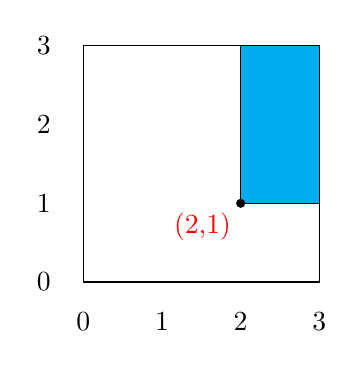
\begin{tikzpicture}
      \draw[step=1cm,black,thin] (0,0) rectangle (3,3);
      \foreach \xtick in {0,...,3} {\pgfmathsetmacro\result{\xtick * 1} \node at (\xtick,-0.5) {\pgfmathprintnumber{\result}}; }
      \foreach \ytick in {0,...,3} {\pgfmathsetmacro\result{\ytick * 1} \node at (-.5,\ytick) {\pgfmathprintnumber{\result}}; }
      \draw[fill=cyan] (2,1) rectangle (3,3);
      \draw [fill=black, thin] (2,1) circle [radius=0.05] node[below left,color=red]{(2,1)};
   \end{tikzpicture}
   \caption{Bottom-left corner example}
\end{figure}

\subsubsection*{Top-right corners} \label{sec:top-right-corners}
As \nameref{sec:bottom-left-corners} but representing the top-right corner of each rectangle (\texttt{tr\_corners}). It is used to reduce the number of positions in which a rectangle can fall in, because it must be inside the bounding box.

To reduce the search space, \texttt{tr\_corners} variables domain is defined as follows: $$\min({\min({px}), \min({py})}) \dots \max({h, w})$$

\begin{figure}[h]
   \centering
   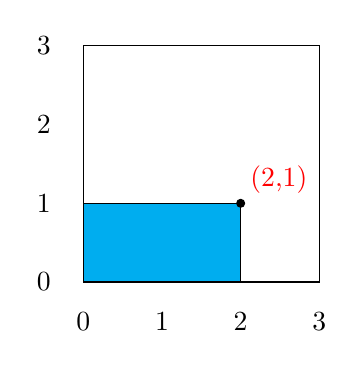
\begin{tikzpicture}
      \draw[step=1cm,black,thin] (0,0) rectangle (3,3);
      \foreach \xtick in {0,...,3} {\pgfmathsetmacro\result{\xtick * 1} \node at (\xtick,-0.5) {\pgfmathprintnumber{\result}}; }
      \foreach \ytick in {0,...,3} {\pgfmathsetmacro\result{\ytick * 1} \node at (-.5,\ytick) {\pgfmathprintnumber{\result}}; }
      \draw[fill=cyan] (0,0) rectangle (2,1);
      \draw [fill=black, thin] (2,1) circle [radius=0.05] node[above right,color=red]{(2,1)};
   \end{tikzpicture}
   \caption{Top-right corner example}
\end{figure}

\subsubsection*{Bottom-left corners values} \label{sec:bottom-left-corners-values}
This is a list of decision variables representing a linearization of bottom-left corners (\texttt{bl\_corners\_values}), which uses a one-to-one mapping from each two-dimensional coordinate in the bounding box to an integer value.

The mapping operates as follows:
$$ c: (x,y) \mapsto x+(y\cdot m),$$ where $m = \max{(h,w)}$.

To reduce the search space, \texttt{bl\_corners\_values} variables domain is defined as follows: $$0 \dots c(w, h)$$

\begin{figure}[h]
   \centering
   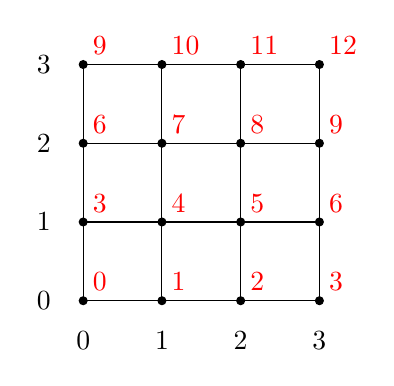
\begin{tikzpicture}
      \draw[step=1cm,black,thin] (0,0) grid (3,3);
      \foreach \xtick in {0,...,3} {\pgfmathsetmacro\result{\xtick * 1} \node at (\xtick,-0.5) {\pgfmathprintnumber{\result}}; }
      \foreach \ytick in {0,...,3} {\pgfmathsetmacro\result{\ytick * 1} \node at (-.5,\ytick) {\pgfmathprintnumber{\result}}; }
      \foreach \x in {0,...,3} {\foreach \y in {0,...,3} {\draw [fill=black, thin] (\x,\y) circle [radius=0.05] node[above right,color=red] {\pgfmathparse{\x+\y*3} \pgfmathprintnumber{\pgfmathresult}};}}
   \end{tikzpicture}
   \caption{Example of 2D-coordinates linearization in a 3 by 3 box}
\end{figure}

\subsection{Constraints}
The constraints described below, divided by scope, are presented at the top of each section with a simple schema depicting their evolution throughout different models.
The following is a legend explaining how constraints advancement is achieved:
\begin{itemize}
   \item \texttt{A[x]}: Constraint \texttt{A} has been introduced in model number \texttt{x}
   \item \texttt{A[x]} $\rightarrow$ \texttt{B[y]}: Constraint \texttt{A} was removed in favor of \texttt{B}, in model \texttt{y}
   \item \texttt{A[x]} $\rightarrow$ \xmark: Constraint \texttt{A} has not been carried over to models \texttt{x + 1, \dots}
\end{itemize}
Model numbers are related to their organization inside the attached Jupyter notebook.

\subsubsection{Non-overlapment}
\begin{itemize}
   \item \nameref{sec:presents-cannot-overlap} $\rightarrow$ \nameref{sec:diffnk}
   \item \nameref{sec:different-bl-corners}
\end{itemize}

\subsubsubsection{Presents cannot overlap [1]} \label{sec:presents-cannot-overlap}
The idea behind this simple constraint is, given a rectangle, to avoid the existance of areas of overlap with every other rectangle.
\begin{gather*}
   \max({bx_{i}, bx_{j}}) \geq \min({bx_{i} + px_{i}, bx_{j} + px_{j}}) \\
   \vee \\
   \max({by_{i}, by_{j}}) \geq \min({by_{i} + py_{i}, by_{j} + py_{j}}) \\
   \forall{i, j = 1 \dots n \mid j > i}
\end{gather*}

The described constraint has been observed to be efficient enough for relatively small instances of the problem, while already suffering to position rectangles in a $17 \times 17$ bounding box. Results are justified by the disjunctive nature of the constraint, which implies an higher burden in the propagation phase.

\subsubsubsection{Global \texttt{diffn\_k} [3]} \label{sec:diffnk}
The \texttt{diffn\_k} global constraint is defined by the official MiniZinc documentation \cite{minizinc} as follows: \\
\emph{Constrains k-dimensional boxes to be non-overlapping. For each box i and dimension j, box\_posn[i, j] is the base position of the box in dimension j, and box\_size[i, j] is the size in that dimension. Boxes whose size is 0 in any dimension still cannot overlap with any other box.}
\begin{verbatim}
   constraint diffn_k(bl_corners, presents);
\end{verbatim}
Being a global constraint, it gives a stronger propagation and a more efficient search w.r.t to \nameref{sec:presents-cannot-overlap}, allowing us to solve bigger instances, up to a $23 \times 23$ bounding box.

It's also notable, as described by \cite{sweep}, that \texttt{diffn\_k} is an onerous constraint. In \cite{sweep} it accounts for 30 to 80\% of the total running time, in an implementation of the \emph{PSP (Perfect Square Packing)} problem, which is very much related to \emph{PWP}.

\subsubsubsection{Global \texttt{all\_different} [2]} \label{sec:different-bl-corners}
The \texttt{all\_different} global constraint asserts that every variable has a different value assigned to it.

In our models it is used w.r.t \texttt{bl\_corners\_values} to ensure that every present has different \texttt{bl\_corners}. The choice of the constrained variables is related to their one-dimensional nature, which guarantees compatibility with MiniZinc's implementation of \texttt{all\_different}.
\begin{verbatim}
   constraint alldifferent(bl_corners_values);
\end{verbatim}

\subsubsection{Containment}
\begin{itemize}
   \item \nameref{sec:reduce-presents-domains}
   \item \nameref{sec:areas-summation}
\end{itemize}

\subsubsubsection{Reduce presents domains [1]} \label{sec:reduce-presents-domains}
The original description is the following one, where the lenght $l$ corresponds to the height \texttt{h\_paper} of the bounding box.:\\
\emph{In any solution, if we draw a vertical line and sum the vertical sides of the traversed pieces, the sum can be at most l. A similar property holds if we draw a horizontal line.}

As suggested by the assignment, we implemented this simple implied constraint which avoids pieces overflow in both directions.
\begin{gather*}
   bx_{i} \leq w + px_{i} \wedge by_{i} \leq h + py_{i}, \forall{i = 1 \dots n}
\end{gather*}

\subsubsubsection{Areas summation [4]} \label{sec:areas-summation}
This implied constraint is used to enforce presents to occupy the entire bounding box, without any kind of wasted space.
In particular, presents areas computed by using top-right and bottom-left corners are linked to the areas calculated using input pieces dimensions.

\begin{gather*}
   \sum_{i=1}^{n} (tx_{i} - bx_{i}) \cdot (ty_{i} - by_{i}) \leq w \cdot h
\end{gather*}
\begin{gather*}
   \sum_{i=1}^{n} (tx_{i} - bx_{i}) \cdot (ty_{i} - by_{i}) = \sum_{i=1}^{n} (px_{i} \cdot py_{i}) 
\end{gather*}

\subsubsection{Positioning}
\begin{itemize}
   \item \nameref{sec:present-at-origin}
   \item \nameref{sec:intervals-approach} $\rightarrow$ \xmark
   \item \nameref{sec:anchor-points-v1} $\rightarrow$ \nameref{sec:anchor-points-v2}$\rightarrow$ \xmark
\end{itemize}

\subsubsubsection{Global \texttt{count\_eq} [2]} \label{sec:present-at-origin}
This implied constraint exploits again the usage of bottom-left corners linearization, i.e. \texttt{bl\_corners\_values},
by simply stating that one and only one present should be placed with its bottom-left corner at the origin.

\begin{gather*}
   \lvert\{\,i \mid bx_{i} = 0 \wedge by_{i} = 0\,\}\rvert = 1
\end{gather*}

\subsubsubsection{Intervals approach [5]} \label{sec:intervals-approach}
It represents an idea taken from \cite{rect-packing}, where domains associated with the $x$-coordinate of bottom-left corners are reduced on the basis of a variable-sized interval:\\
\emph{[...] a rectangle is assigned an interval of x-coordinates. Interval sizes are hand-picked for each rectangle prior to search, and they induce a smaller rectangle representing the common intersecting area of placing the rectangle in any location in the interval. [...] we assign all x-coordinates prior to any y-coordinates, and use interval variables for the x-coordinates. We set a rectangle’s interval size to 0.35 times its width, which gave us the best performance. Finally, we do not use interval variables for the y-coordinates.}

\begin{figure}[h]
   \centering
   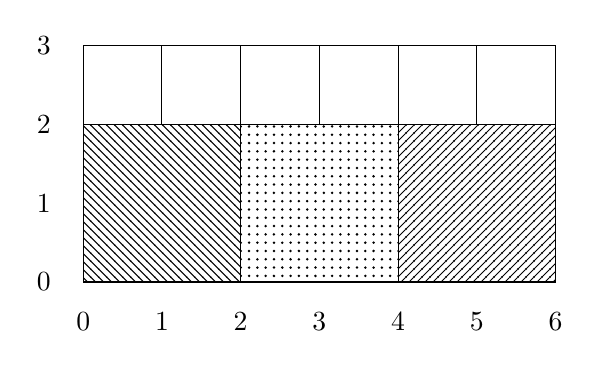
\begin{tikzpicture}
      \draw[step=1cm,black,thin] (0,2) grid (6,3);
      \foreach \xtick in {0,...,6} {\pgfmathsetmacro\result{\xtick * 1} \node at (\xtick,-0.5) {\pgfmathprintnumber{\result}}; }
      \foreach \ytick in {0,...,3} {\pgfmathsetmacro\result{\ytick * 1} \node at (-.5,\ytick) {\pgfmathprintnumber{\result}}; }
      \draw[pattern=south east lines, pattern color=black] (0,0) rectangle (2,2);
      \draw[pattern=dots, pattern color=black] (2,0) rectangle (4,2);
      \draw[pattern=south west lines, pattern color=black] (4,0) rectangle (6,2);
   \end{tikzpicture}
   \caption{Intervals example: assigning a $4\times2$ to $[0,2]$}
   \label{fig:intervals}
\end{figure}

As shown in figure \ref{fig:intervals}, a $4\times2$ rectangle assigned an $x$-interval of $[0,2]$ consumes 2 units of area at each $x$-cordinate in $[2,3]$, represented by the dotted area.

If there were no feasible set of interval assignments, then the constraint would save us from having to try individual $x$ values. However, if we do find a set of interval assignments, then we must search for a set of single $x$-coordinate values.

\subsubsubsection{Anchor points [5]} \label{sec:anchor-points-v1}
It represents a reduction on each present's domain, such that bottom-left corners reside on corners of other rectangles or on the wrapping paper borders.

The main implementation-wise problem was our inability of correctly expressing the constraint in an efficient way: the only thing we were able to describe is an upper bound on the number of the overall distinct corners that can be found inside the bounding box at the same time, while also satisfying every other constraint.
To do that, a new list of decision variables had to be created (\texttt{corners\_values}), containing the linearization (as in \ref{sec:bottom-left-corners-values}) of every corner for each present. 
The constraint was then posted by limiting unique values, i.e. unique corners, and by forcing each bounding box corner to coincide with exactly one corner, over this new list of variables.

\begin{verbatim}
   constraint nvalue(corners_values) <= 2 * n + 2
\end{verbatim}

\subsubsubsection{Anchor points [6]} \label{sec:anchor-points-v2}
This constraint is an evolution of \nameref{sec:anchor-points-v1}, which introduces a more coincise and efficient anchor points approach.
This time the main idea is about causing the bottom-left corner of a single rectangle to fit a bottom-left corner of another rectangle or a top-left corner of another rectangle, thus reducing the amount of available presents positions combinations inside the wrapping paper.

\begin{gather*}
   bx_{i} \in \{\,0\,\} \cup \{\, bx_{j} + px_{j} \mid j = 1 \dots i - 1, i + 1, \dots n \,\} \\
   \wedge \\
   by_{i} \in \{\,0\,\} \cup \{\, by_{j} + py_{j} \mid j = 1 \dots i - 1, i + 1, \dots n \,\} \\
   \forall{i = 1 \dots n}
\end{gather*}

The described formula was implemented using the global constraint \texttt{member}, so as to achieve better propagation. 

The constraint was later removed from the CP model, since it didn't seem to make any major difference, at least w.r.t. running times over the test instances, even though it was implemented using a global constraint.

\begin{figure}[h]
   \centering
   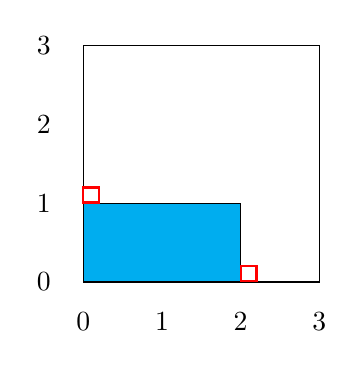
\begin{tikzpicture}
      \draw[step=1cm,black,thin] (0,0) rectangle (3,3);
      \foreach \xtick in {0,...,3} {\pgfmathsetmacro\result{\xtick * 1} \node at (\xtick,-0.5) {\pgfmathprintnumber{\result}}; }
      \foreach \ytick in {0,...,3} {\pgfmathsetmacro\result{\ytick * 1} \node at (-.5,\ytick) {\pgfmathprintnumber{\result}}; }
      \draw[fill=cyan] (0,0) rectangle (2,1);
      \draw[color=red, thick] (2,0.01) rectangle (2.2,0.2);
      \draw[color=red, thick] (0,1.01) rectangle (0.2,1.2);
   \end{tikzpicture}
   \caption{Anchor points example}
\end{figure}

\subsubsection{Stacking}
\begin{itemize}
   \item \nameref{sec:cumulative}
   \item \nameref{sec:stack-two} $\rightarrow$ \nameref{sec:column-stacking}
\end{itemize}

\subsubsubsection{Global \texttt{cumulative} [3]} \label{sec:cumulative}
\begin{figure}
   \centering
   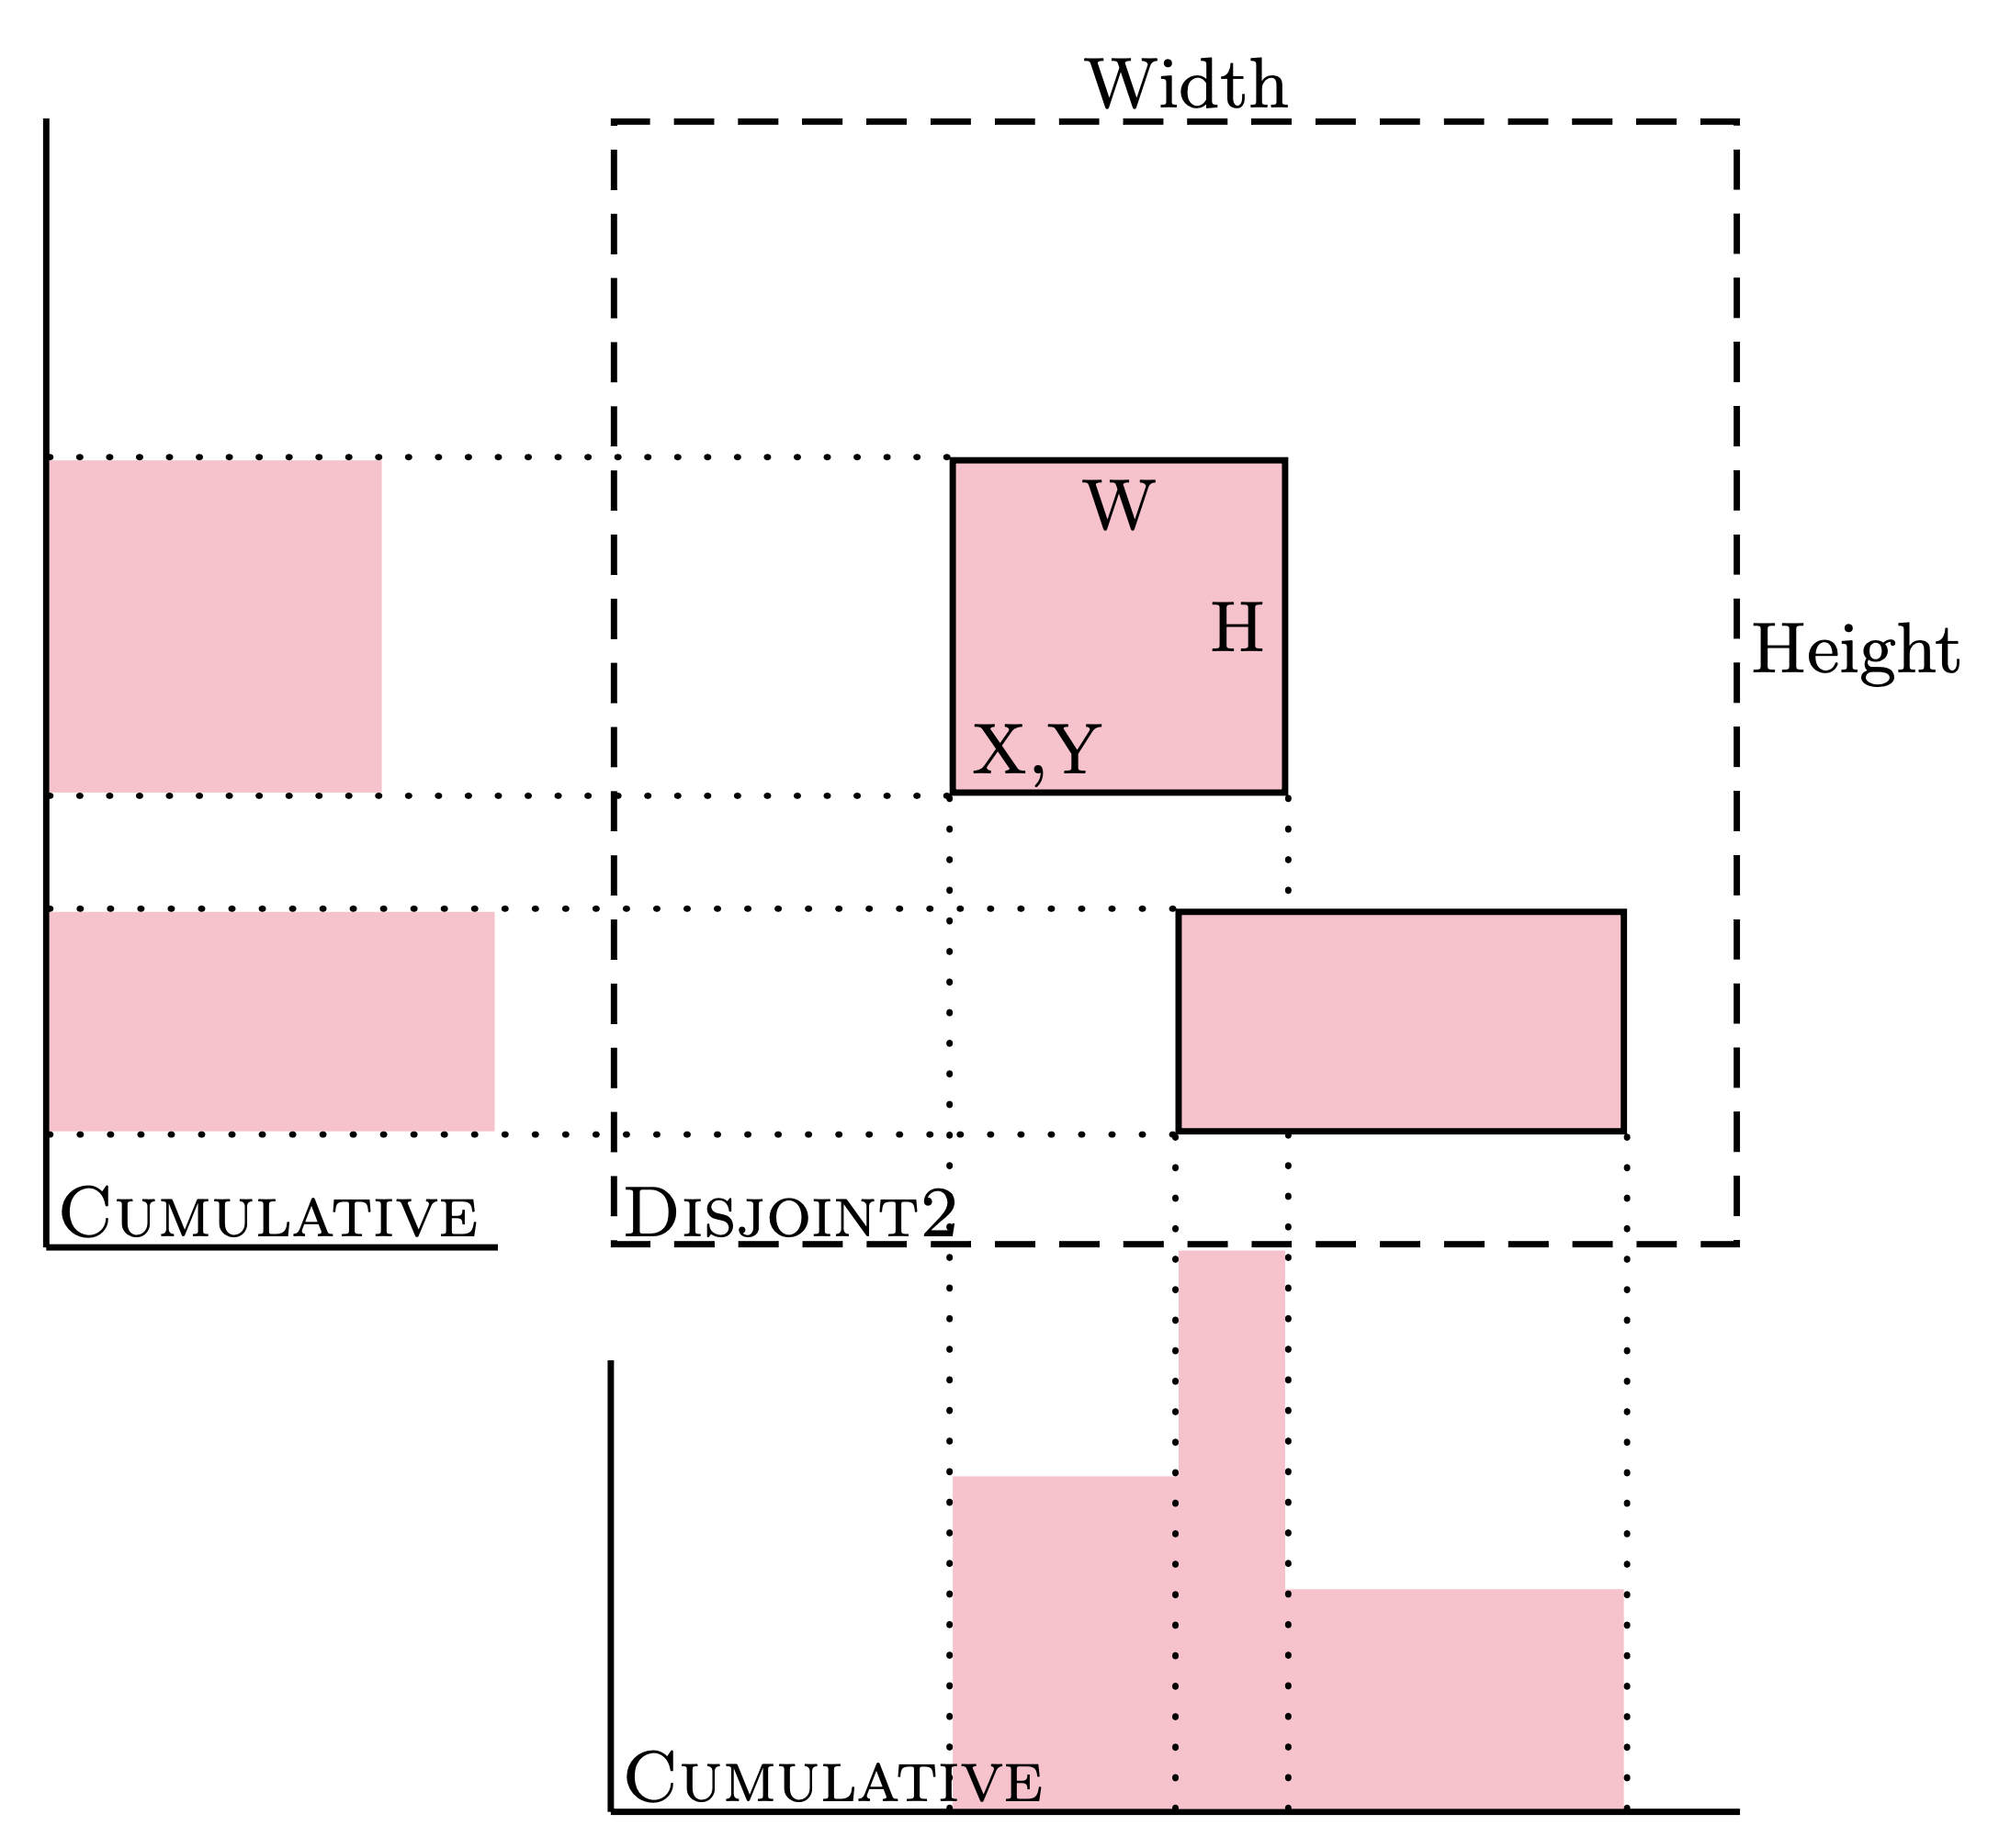
\includegraphics[scale=0.2]{cumulative.png}
   \caption{Cumulative global constraint (image taken from \cite{cumulative})}
\end{figure}

\subsubsubsection{Column stacking by two [4]} \label{sec:stack-two}
\subsubsubsection{General column stacking [5]} \label{sec:column-stacking}

\subsubsection{Symmetry breaking}
\begin{itemize}
   \item \nameref{sec:biggest-lower-left} $\rightarrow$ \nameref{sec:areas-ordering}
   \item \nameref{sec:width-ordering} $\rightarrow$ \xmark
\end{itemize}

\subsubsubsection{Biggest rectangle in lower left quadrant [4]} \label{sec:biggest-lower-left}
\subsubsubsection{Ordering by areas [6]} \label{sec:areas-ordering}
\subsubsubsection{In-column ordering by width [4]} \label{sec:width-ordering}


\subsection{Models}

\subsubsection*{Search strategy}

\section{Satisfiability Modulo Theory}

\printbibliography

\end{document}
